\chapter{Opis projektu i implementacji}
\label{cha:rozdzial5}

\section{Wprowadzenie}

W ramach projektu powstał odtwarzacz multimedialny umożliwiający adaptację strumieniowania w oparciu o standard DASH-MPEG. Poniższy rozdział zawiera informacje opisujące algorytm wykorzystany do implementacji strumieniowania adaptacyjnego. Pomysł algorytmu oparty o wykorzystanie strukturę kontrolera PID został zaczerpnięty z artykułu "Towards Agile and Smooth Video Adaptation in Dynamic HTTP Streaming"~\cite{Tian}. Dalsza część rozdziału skupia się na szczegółach implementacyjnych odtwarzacza oraz narzędziach i bibliotekach wykorzystanych do jego stworzenia.

\section{Opis algorytmu}
\label{sec:alg}

Prezentowany poniżej algorytm służy do wygładzenia procesu adaptacji strumienia danych multimedialnych. Oznacza to, że przy dużej zmienności warunków panujących w sieci alogrytm będzie starał utrzymać jakość przesyłanych danych (reprezentację) na stabilnym poziomie. 

Branie pod uwagę jedynie dostępnej przepustowości z danej chwili podczas wyboru konkretnej reprezentacji danych może prowadzić do ciągłych i widocznych dla użytkownika zmian w jakości oglądanego materiału. Oparcie algorytmu na idei kontrolera PID pozwala na kompensację różnic pomiędzy wartością dostępnej przepustowości oraz bitrate wybranej reprezentacji i zwiększa jego tolerancję na chwilowe zmiany w dostępnym paśmie. Kontroler PID wykorzystuje pętlę sprzężenia zwrotnego i składa się z trzech komponentów:
\begin{itemize}
\item P \textit{(proportional)} - odpowiada za kompensację różnicy bieżącej,
\item I \textit{(integral)} - kompensuje akumulację różnic z przeszłości,
\item D \textit{(derivative)} - kompensuje przyszłe przewidywane różnice.
\end{itemize}
Ogólna zasada działania mechanizmu adaptacji została przedstawiona na rysunku~\ref{fig:PID} oraz w tabeli objaśniającej wykorzystane oznaczenia~\ref{PID_table}. Dalsza część podrozdziału została podzielona na sekcje opisujące wybrane elementy zaimplementowanego rozwiązania.

\begin{figure}[h!]
	\centering
		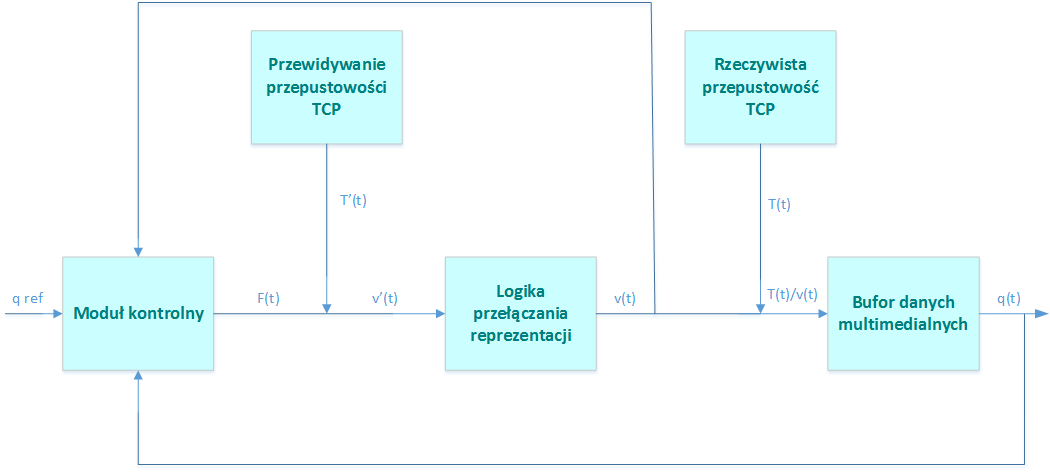
\includegraphics[width=\linewidth]{PID}
	\caption{Schemat adaptacji w oparciu o kontroler PID, na podstawie: \cite{Tian}}
	\label{fig:PID}
\end{figure}

\begin{figure}
	\centering
	\begin{tabular}{ c | c }
  		Oznaczenie & Objaśnienie \\
  		\hline
  		q ref	&  referencyjna (docelowa) zajętość bufora danych. \\
		F(t)	&  czynnik adaptacji. \\
		T'(t)	&  przewidywana przepustowość w chwili t. \\
		v'(t)	&  przewidywany bitrate danych multimedialnych. \\
		v(t)	&  bitrate danych po adaptacji i kwantyzacji.\\
		T(t)	&  zmierzona przepustowość w chwili t.\\
		q(t)	&  poziom zajętości bufora danych w chwili t. \\
	\end{tabular}
	\caption{Tabela oznaczeń z rysunku \ref{fig:PID}.}
	\label{PID_table}
\end{figure}

\subsection{Moduł kontrolny}

Moduł kontrolny wykorzystuje kilka parametrów do wyliczenia czynika adaptacji \textit{F(t)} potrzebnego do ustalenia wstępnego bitrate danych \textit{v'(t)}. Czynnik adaptacji \textit{F(t)} jest iloczynem dwóch wartości:
\begin{itemize}
\item \textit{Czynnik zajętości bufora} - liczony na podstawie zajętości referencyjnej \textit{q ref} oraz zajętości rzeczywistej \textit{q(t)}. Im większa różnica pomiędzy tymi dwoma wielkościami, tym większa będzie szybkość adaptacji. W wypadku, gdy wartości będą zbliżone lub równe, powyższy czynnik będzie miał neutralny wpływ na wartość czynnika adaptacji. 
\item \textit{Czynnik trendu bufora} - obliczany na postawie kolejnych wartości \textit{q(t)}. Jeżeli w danych w buforze przybywa to jest to sygnał do zwiększenia wartości czynnika trendu bufora. Jeżeli bufor jest opróżniany to ten czynnik odpowiednio maleje. Utrzymywanie się poziomu zajętości bufora na jednakowym poziomie powoduje, że trend bufora nie wpływa na wartość czynnika adaptacji.
\end{itemize}

\subsection{Przewidywanie przepustowości TCP}

Algorytm ma do dyspozycji dwa sposoby przewidywania przyszłej przepustowości łącza TCP. Możliwy jest wybór metody predykcji podczas uruchamiania aplikacji odtwarzacza multimedialnego.

Pierwsze metoda polega na liczeniu średniej z kilku ostatnich przechowywanych pomiarów przepustowości. Odrzucane są skrajne pomiary, a wielkość bufora na przetrzymywane pomiary jest konfigurowalna.

Druga metoda wykorzystuje wykładniczą średnią kroczącą. Zaletą metody jest szybkie dostosowanie się do długofalowych trendów zmian w przepustowości i dodatkowa ochrona przed krótkotrwałymi zmianami w paśmie.

\subsection{Logika przełączania reprezentacji}

Moduł odpowiedzialny za przełączanie reprezentacji został opisany za pomocą poniższego pseudokodu:

\begin{algorithm}
\label{alg:switch}
\caption{Logika przełączania reprezentacji}
\begin{algorithmic}[1]
\State{$v'(t) = F(t) \cdot T'(t)$}
\If{$q(t) < \frac{q_{ref}}{2}$}
	\State{$v(t)=Q(T(t-1))$}
	\State{$return$}
\ElsIf{$v'(t) > v(t-1)$}
	\State{$Counter++$}
	\If{$Counter>m$}
		\State{$v(t)=Q(T'(t))$}
		\State{$Counter=0$}
		\State{$return$}
	\EndIf
\ElsIf{$v'(t)<v(t-1)$}
	\State{$Counter=0$}
\EndIf
\State{$v(t)=v(t-1)$}
\State{$return$}
\end{algorithmic}
\end{algorithm}

Funkcja Q jest funkcją kwantyzacji. Bitrate \textit{v'(t)} obliczany na podstawie przewidywanej przepustowości oraz czynnika adaptacji (pierwsza linia) może przyjmować dowolne wartości. Istnieje jednak skończona liczba reprezentacji o okreśonych wartościach bitrate. Funkcja Q odwzorowuje dowolny bitrate na wartość największą, ale nie większą niż argument funkcji i pochodzącą ze zbioru składającego się z bitrate dostępnych reprezentacji. W drugiej linii aktualny poziom bufora jest porównywany z poziomem referencyjnym i jeżeli będzie co najmniej dwukrotnie mniejszy to istnieje ryzyko, że z bufora wyciągnięte zostaną wszystkie dane multimedialne. W celu redukcji tego zagrożenia za wynikowy bitrate przyjmowana jest skwantyzowana wartość rzeczywistej przepustowości zmierzona podczas pobierania poprzedniego segmentu danych. 

Jeżeli warunek z linii 2 nie zachodzi to w następnej kolejności sprawdzane jest czy przewidywany bitrate jest większy niż bitrate ostatnio pobranego segmentu (linia 5). Za każdym razem gdy warunek z linii nr 5 jest spełniony, zwiększana jest wartość licznika \textit{Counter}, który po przekroczeniu wartości \textit{m} jest zerowany, a wynikowy bitrate jest ustalany jako skwantyzowana wartość przewidywanej przepustowości (linia 8). 

Jeżeli warunki z linii 2 i 5 nie są spełnione to sprawdzane jest czy przewidywany bitrate jest mniejszy od bitrate poprzednio pobranego segmentu. Jeżeli tak to licznik jest zerowany, a wynikowy bitrate jest taki sam jak w poprzedniej iteracji algorytmu. 

\section{Wysokopoziomowa koncepcja rozwiązania}

Odtwarzacz multimedialny składa się z 4 komponentów przedstawionych na rysunku \ref{fig:ImplementationConceptual}. 

\begin{figure}[h!]
	\centering
		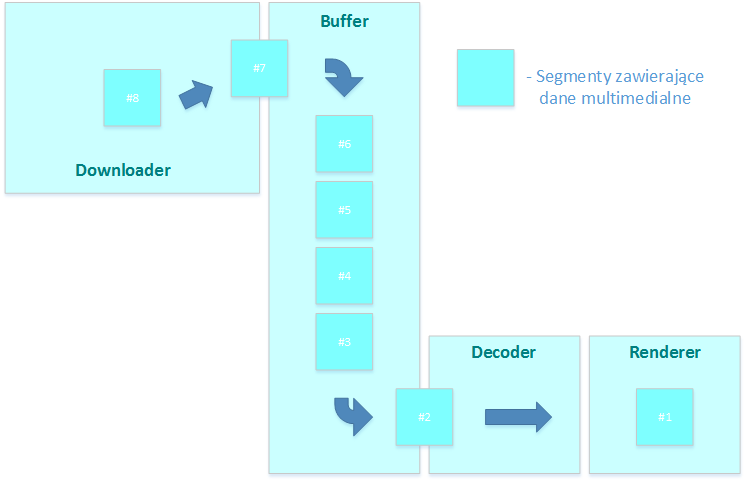
\includegraphics[width=\linewidth]{ImplementationConceptual}
	\caption{Koncepcja rozwiązania}
	\label{fig:ImplementationConceptual}
\end{figure}

Pierwszy z komponentów, \textit{Downloader}, odpowiada za komunikację z serwerem HTTP na którym znajdują się dane multimedialne przeznaczone do strumieniowania. Jest różnież odpowiedzialny za zbieranie danych związanych z transmisją:
\begin{itemize}
\item czas rozpoczęcia pobierania segmentu danych,
\item czas zakończenia pobierania segmentu danych,
\item wielkość pobranego segmentu danych,
\item pozostałe elementy metryki wyszczególnione w standardzie DASH-MPEG.
\end{itemize}
Downloader po zakończeniu pobierania segmentu danych multimedialnych przekazuje go do bufora. 

Ze względu na wielowątkowość aplikacji, bufor synchronizuje dostęp do 
przechowywanych segmentów danych multimedialnych. Architektura wykorzystująca model producenta i konsumenta pozwala na niezależne działanie komponentu \textit{Downloader} i komponentów zajmujących się przetwarzaniem i prezentacją danych. 

Dane multimedialne są wyjmowane z bufora i dekodowane - zajmuje się tym \textit{Decoder}. Po przetworzeniu dane przekazywane są do komponentu \textit{Renderer} odpowiedzialnego za prezentację zdekodowanych danych użytkownikowi.

\section{Implementacja projektu odtwarzacza}

\begin{sidewaysfigure}
	\centering
		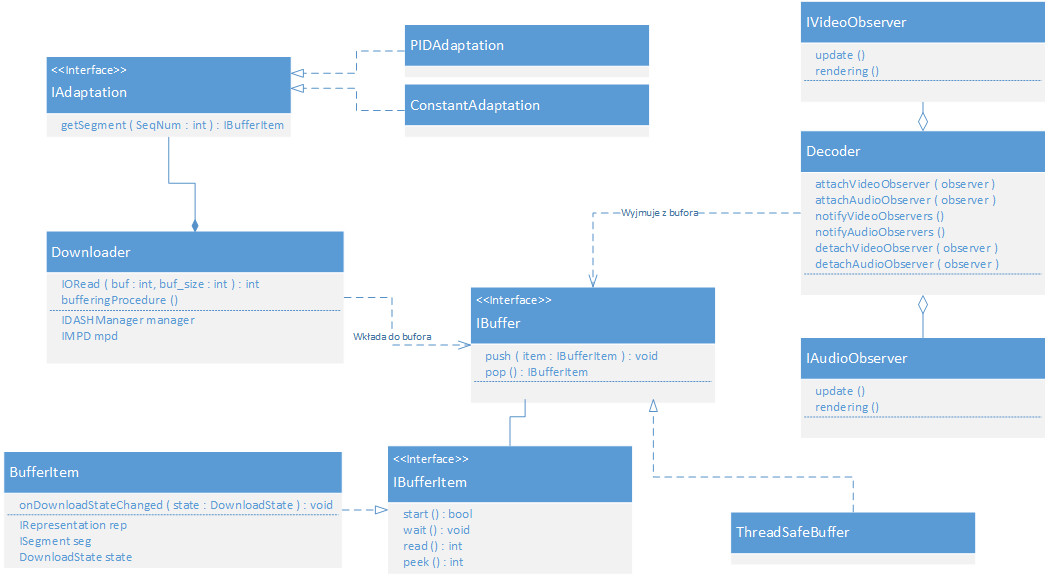
\includegraphics[scale=0.8]{Class}
	\caption{Diagram klas}
	\label{fig:Class}
\end{sidewaysfigure}

Diagram klas na rysunku \ref{fig:Class} przedstawia najważniejsze klasy i powiązania pomiędzy nimi. Poniższy podrozdział skupia się na wyjaśnieniu przeznaczenia poszczególnych klas oraz ich wzajemnych zależności.

Obiekt klasy \textit{Downloader} jest odpowiedzialny za komunikację z serwerem HTTP i pobieraniem kolejnych segmentów danych multimedialnych. Podczas uruchamiania odtwarzacza należy podać lokalizację pliku MPD (Media Presentation Description), który następnie jest pobierany i parsowany przez obiekt implementujący interfejs \textit{IDASHManager} należący do biblioteki libdash. Pobieranie konkretnego segmentu jest delegowane do osobnego wątku wykonującego instrukcje funkcji \textit{bufferingProcedure}. W celu wybrania reprezentacji z której należy skorzystać przy pobieraniu segmentu danych multimedialnych \textit{Downloader} korzysta z klas implementujących \textit{IAdaptation}. Segmenty, których pobieranie zakończyło się sukcesem wkładane są do bufora implementującego interfejs \textit{IBuffer}. 

Logika adaptacji strumienia polegająca na wyborze kolejnej wersji danych multimedialnych (ich reprezentacji) jest zawarta w klasach implementujących interfejs \textit{IAdaptation}. Obiekt klasy \textit{Downloader} korzysta z funkcji \textit{getSegment} w celu uzyskania nowego obiektu implementującego interfejs \textit{BufferItem}, który na obecnym etapie cyklu życia reprezentuje jeszcze nie pobrany segment danych. Obiekty klas implementujących \textit{IAdaptation} zajmują się wyborem reprezentacji, tworzeniem nowego obiektu obudowującego wybrany segment danych oraz przekazaniem go do obiektu \textit{Downloader}. Odtwarzacz pozwala na wybór algorytmu adaptacji. Obecnie możliwy jest wybór jednego z dwóch mechanizmów adaptacji:
\begin{itemize}
\item \textit{InteractiveAdaptaion} - pozwala na sterowanie wyborem reprezentacji w czasie rzeczywistym. Możliwy jest wybór dowolnej z reprezentacji opisanych w pliku MPD, którego lokalizacja została podana przy starcie odtwarzacza. W przypadku wyboru nieprawidłowej reprezentacji, odtwarzacz zwraca informację o błędzie i pracuje z wykorzystaniem poprzedniej reprezentacji.
\item \textit{ConstantAdaptation} - wybór reprezentacji należy podać przy uruchamianiu odtwarzacza i pozostaje on niezmienny przez cały czas działania aplikacji. Jeżeli reprezentacja nie znajduje się w zbiorze dostępnych reprezentacji opisanych plikiem MPD to aplikacja odtwarzacza zostaje zamknięta i zwrócona zostaje informacja o błędzie.
\item \textit{PIDAdaptaion} - adaptacja strumienia opierająca się o kontroler PID i algorytm opisany w podrozdziale \ref{sec:alg}. Adaptacja zachodzi automatycznie i nie wymaga interwencji użytkownika.
\end{itemize}

Obiekty klas implementujących \textit{IBufferItem} stanowią kontener na dane pobierane z serwera. Składają się przede wszystkim z obiektów klas należących do biblioteki libdash oraz zawierają stan pozwalający na stwierdzenie, czy segment, który obiekt reprezentuje został już pobrany. Można na nich wykonywać operacje rozpoczęcia pobierania (\textit{start}), oczekiwania na zakończenie pobierania (\textit{wait}) oraz operacje podglądania danych w segmencie i ich czytania.

Klasa \textit{ThreadSafeBuffer} stanowi implementację interfejsu \textit{IBuffer}. Obiekt tej klasy pozwala na synchronizowany dostęp wielu wątków do kolejki zawierającej elemnty implementujące \textit{IBufferItem}. Wykorzystany został współbieżny wzorzec projektowy producent-konsument. Producentem jest obiekt klasy \textit{Downloader}, natomiast konsumentami mogą być obiekty typu \textit{Decoder}. Procedura \textit{push} pozwala na wkładanie elementów na początek bufora, natomiast procedura \textit{pop} zwraca ostatni element przy okazji usuwając go z bufora.

\textit{Decoder} zajmuje się dekodowaniem danych zawartych w kolejnych segmentach. Po zdekodowaniu segmentu danych multimedialnych powiadamiane są obiekty odpowiedzialne za prezentację danych użytkownikowi. Klasy obiektów odpowiedzialnych za prezentację implementowane są jako obserwatory obiektów klasy \textit{Decoder}. \textit{Decoder} pozwala na rejestrację i odrejestrowanie wielu obiektów pozwalających na renderowanie danych audio oraz video.

\section{Wykorzystane narzędzia i biblioteki}

Projekt odtwarzacza powstał w języku C++ i z wykorzystaniem Microsoft Visual Studio 2010. Budowanie aplikacji odbywa się za pomocą programu CMake. Odtwarzacz korzysta z bibliotek libav, libcurl, libxml2, sdl, zlib, boost oraz biblioteki libdash implementującej standard DASH-MPEG. Wykorzystany został system kontroli git.

